\chapter{Dynamique du point}
\label{chapter2}

\textit{Grâce au premier chapitre, nous sommes en mesure de décrire le mouvement d'un objet via sa position, sa vitesse et son accélération. Dans ce second chapitre nous allons nous intéresser aux causes des mouvements des objets : les forces. Nous verrons alors qu'il est possible de prédire le mouvement d'un objet en connaissant les forces qui s'y appliquent : c'est ce qu'on appelle la dynamique. Grâce à cette dernière, la mécanique prend un aspect divinatoire.}

\section{Principe fondamental de la dynamique}

\subsection{Énoncé}

\paragraph{}En mécanique classique, un objet de masse $m$ soumis à une force $\vv{F}$ possède une accélération $\vv{a}$ telle que :

\begin{equation}
	\vv{F} = m\vv{a},\quad \text{ou} \quad \vv{a} = \frac{\vv{F}}{m}
	\label{eq:pfd}
\end{equation}

\noindent On appelle l'\autoref{eq:pfd} \textbf{principe fondamental de la dynamique} (PFD), énoncé par Isaac Newton\footnote{Vous connaissez peut-être déjà ce principe sous le nom de seconde loi de Newton}. Dans la suite, nous allons voir que ce principe est en fait assez intuitif.

\subsection{La masse}

\paragraph{}Tous les objets ne se comportent pas de la même façon face à la mise en mouvement. En effet, même en appliquant le même effort dans sa raquette, il est beaucoup plus compliqué de renvoyer une balle de pétanque qu'une balle de ping pong. C'est ce qu'on appelle le phénomène d'inertie, certains objets résistent plus à la mise en mouvement que d'autres.

\paragraph{}De manière intuitive, on peut qualifier l'inertie d'un objet par sa masse. La masse est donc une grandeur positive qui qualifie la résistance à la mise en mouvement. Plus un objet est lourd (la balle de pétanque par exemple), plus il résiste à la mise en mouvement. À l'inverse, plus un objet est léger (la balle de ping pong par exemple), plus il peut être mis en mouvement facilement. La masse s'exprime en kilogrammes (\SI{}{\kg}).

\paragraph{}Cette définition de la masse se retrouve directement dans le PFD. En effet, en termes de normes on a :

\begin{equation}
	a = \frac{F}{m}
	\label{eq:PFDnorm}
\end{equation}

\noindent et donc plus la masse de l'objet est grande plus, à force égale, l'accélération de l'objet est faible et donc sa mise en mouvement peu efficace.

\subsection{Notion de force}

\paragraph{}Les modifications sur le mouvement d'un objet (mise en mouvement ou changement du mouvement déjà en cours) sont dues à des interactions avec l'environnement extérieur. Pour modéliser ces interactions, on utilise la notion de force : 

\begin{defi}{Force}
	Une force est une grandeur vectorielle, dont la norme s'exprime en Newton (\SI{}{\newton}), qui décrit l'interaction capable de modifier le mouvement d'un objet.
\end{defi}

\paragraph{}Le caractère vectoriel d'une force apparaît de manière assez évidente. En effet, l'interaction doit être définie par une direction, un sens et une intensité. Par exemple, si je tire sur un ressort, la force exercée par ce ressort sur ma main se fait dans la direction d'élongation du ressort, dans le sens de repli du ressort, et cette force est d'autant plus intense que le ressort a été étiré. Sans caractère vectoriel de cette grandeur, on ne sait pas dans quelle direction l'objet soumis à la force est tiré (ou bien repoussé).

\paragraph{}Si l'on regarde en termes de norme le PFD (voir \autoref{eq:PFDnorm}), on remarque que l'accélération d'un objet est d'autant plus grande que la norme de la force (et donc son intensité) est grande. Cela est tout à fait intuitif : plus on frappe fort la balle de ping pong avec notre raquette, plus celle-ci va être accélérée.

\subsection{Système soumis à plusieurs forces}


\paragraph{}Dans le cas où le système étudié est soumis à plusieurs forces, le PFD se généralise en considérant la somme vectorielle de toutes les forces $\vv{F}_i$ en jeu :

\begin{equation}
	\sum_i \vv{F_i}=m\vv{a}
\end{equation}

\paragraph{}\textit{Le principe fondamental de la dynamique est donc un principe très simple qui relie les interactions extérieures sur un objet et le mouvement de celui-ci. Malgré sa simplicité, son interprétation se révèle en fait très riche.}

\subsection{Utilisation du principe fondamental de la dynamique}

\subsubsection{Détermination du mouvement d'un objet}

\paragraph{}Grâce au PFD, si l'on connaît les différentes forces s'appliquant sur un objet, on est capable de connaître l'accélération de ce dernier. Or dans le premier chapitre, nous avons vu que, de l'accélération, nous pouvons tirer la vitesse et la position de l'objet. Ainsi, simplement à partir des forces extérieures, nous sommes capable de prédire le mouvement de l'objet. C'est là tout le sujet de la dynamique newtonienne.

\paragraph{}Dans la partie suivante, nous verrons quelques exemples de prédictions de mouvement basées sur ce principe.

\subsubsection{Systèmes isolés et pseudo-isolés}

\paragraph{}Il existe un cas particulier d'application du PFD, celui dans lequel l'objet étudié n'est soumis à aucune force extérieure (système isolé) ou bien dans lequel la résultante des différentes forces est nulle (système pseudo-isolé). Dans le cas des systèmes isolés ou pseudo-isolés, l'application du PFD nous dit que l'accélération est nulle :

\begin{equation}
	\sum_i \vv{F_i} = \vv{0} \Rightarrow \vv{a} = \vv{0}
\end{equation}

\paragraph{}Par définition de l'accélération (qui est la dérivée du vecteur vitesse), cela signifie qu'un tel système possède un vecteur vitesse constant en direction et en norme. Autrement dit, cela correspond à un mouvement rectiligne uniforme (voir \autoref{chapter1}). Notons par ailleurs que l'immobilité est un cas particulier du mouvement rectiligne uniforme (vitesse uniformément nulle). Ce raisonnement constitue le principe d'inertie :

\begin{defi}{Principe d'inertie}
	Un système isolé ou pseudo-isolé conserve un mouvement rectiligne uniforme. 
\end{defi}

\paragraph{}Si la prédiction d'un mouvement rectiligne uniforme ou l'absence de mouvement n'est pas très intéressant, la réciproque du principe d'inertie peut, elle, s'avérer utile. Par exemple, si l'on sait qu'un objet est immobile, on sait que la résultante des forces s'appliquant sur lui est nulle. De cette manière il est possible de caractériser des forces extérieures !

\subsection{Écueil sur les référentiels galiléens ($\star$)}

\paragraph{}En toute rigueur, le PFD n'est valable que lorsque l'on se place dans un référentiel galiléen. Toutefois, nous ne considérerons dans ce cours que des référentiels galiléens et omettront donc cette subtilité. Pour lae lecteurice intéressé-e, il est en fait possible de généraliser le PFD à des référentiels non galiléens en considérant les forces fictives d'inertie qu'ils génèrent. C'est notamment le cas lorsqu'on considère la force centrifuge dans un référentiel en rotation, comme dans le cas d'un manège tournant ou d'une centrifugation différentielle en biologie.

\section{Forces en présence dans le systèmes biologiques}

\paragraph{}\textit{Dans cette partie, nous allons faire l'inventaire de quelques forces omniprésentes en biologie afin de pouvoir prédire le mouvement de systèmes intéressants.}

\subsection{Le poids}

\paragraph{}La force la plus largement étudiée sur Terre est le poids. Le poids est la force d'attraction gravitationnelle dans le cas précis de la Terre. Un objet possédant une masse sur la surface de la Terre ressent une attraction vers le centre de cette dernière (en direction du sol donc) proportionnelle à sa masse. Soit un objet de masse $m$, le poids s'appliquant sur celui-ci s'exprime :

\begin{equation}
	\vv{P} = m \vv{g}
	\label{eq:poids}
\end{equation}

\noindent avec $\vv{g}$ l'accélération de la pesanteur, de norme $g = \SI{9,8}{\meter\per\second\squared}$, et dirigée vers le sol. Sur la \autoref{fig:ballespoids} on représente le poids de différentes balles lancées en l'air. En premier approximation, le poids est une force qui ne varie ni dans l'espace, ni dans le temps. Tout au long du mouvement, un objet est soumis au même poids.

\begin{figure}[h]
	\centering
	\includegraphics[width=0.7\textwidth]{Chapitre2/Figures/PoidsBalles.pdf}
	\caption{Représentation du poids de différentes balles. La masse de la balle de basket est plus grande que celle de la balle de tennis, elle-même plus grande que celle de la balle de ping pong. La norme du poids étant proportionnelle à la masse de l'objet, la norme du poids de la balle de basket est plus grande que celle de la balle de tennis, elle-même plus grande que celle de la balle de ping pong}
	\label{fig:ballespoids}
\end{figure}

\paragraph{}\textit{Dans le langage courant, on confond souvent poids et masse. Ce n'est pas la même chose ! Le poids est une force (s'exprime en \SI{}{\newton}) s'appliquant sur un objet qui a une masse (s'exprime en \SI{}{\kg}). La confusion vient du fait qu'on se sert en général du poids pour mesurer indirectement la masse. En effet, une balance mesure le poids qui s'applique sur un objet et, par conversion, en utilisant l'\autoref{eq:poids}, en déduit la masse.}

\subsection{Force de rappel d'un ressort}

\paragraph{}Une autre force très utilisée en physique est la force de rappel qu'applique un ressort sur un objet collé à son extrémité. Si la longueur à vide du ressort est $l_0$, alors un ressort étiré d'une longueur $l$ applique une force de traction sur son extrémité :

\begin{equation}
	\vv{F_r} = k\Delta l \vv{e_x} = k(l_0-l)\vv{e_x}
	\label{eq:forceressort}
\end{equation}

\noindent avec $k$ la constante de raideur du ressort, s'exprimant en \SI{}{\newton\per\meter} (d'autant plus grande que le ressort est raide) et $\vv{e_x}$ le vecteur unitaire dans le sens de l'élongation du ressort.

\paragraph{}En pratique, on fait rarement face à des problèmes faisant intervenir des ressorts à proprement parler, surtout en biologie. Toutefois, dans bien des cas, il est très pratique de modéliser certains objets par des ressorts afin de représenter la force qu'ils exercent. C'est le cas notamment des pinces optiques, un dispositif expérimental très utilisé en biologie. Une pince optique est un dispositif formée d'un laser focalisé en un point, dont le rayonnement électromagnétique associé va agir comme un piège afin de maintenir un objet au niveau du point focal. La zone de focalisation d'un laser pouvant être réduite à quelques centaines de nanomètres, cet outil permet d'agir sur des objets très petits, comme des organelles à l'intérieur des cellules par exemple. En première approximation, on modélise la force d'attraction associée à une pince optique par la force de rappel d'un ressort (voir \autoref{fig:pinceoptique}). Comme on le verra en TD, cela peut permettre d'étudier des propriétés très intéressantes des systèmes biologiques microscopiques, comme les moteurs moléculaires.

\begin{figure}[h]
	\centering
	\includegraphics[width=0.6\textwidth]{Chapitre2/Figures/pinceoptique.pdf}
	\caption{Modélisation du système de pince optique par un ressort.}
	\label{fig:pinceoptique}
\end{figure}

\subsection{Force de frottements visqueux}

\paragraph{}Si vous l'avez déjà essayé, vous avez sûrement remarquer qu'il est bien plus difficile de courir dans l'eau plutôt que de courir dans l'air. Cela vient du fait que lorsque l'on se déplace dans un milieu matériel, nous sommes soumis à une force de frottements visqueux. Si l'on considère une sphère de rayon $R$ se déplaçant dans un fluide à la vitesse $\vv{v}$, celle-ci est en fait soumise à une force de frottements visqueux $\vv{f}$ de la forme :

\begin{equation}
	\vv{f} = 6\pi\eta R \vv{v}
\end{equation}

\noindent avec $\eta$ la viscosité dynamique du fluide. Comme son nom l'indique, la viscosité dynmaique d'un fludie est d'autant plus grande que le fluide est visqueux. Par exemple, on a $\eta_\text{eau} = \SI{1,00e-3}{\pascal \second}$ et $\eta_\text{miel}=\SI{10}{\pascal\second}$

\paragraph{}D'après cette expression, on remarque donc bien que cette force s'oppose au mouvement de l'objet puisque son sens est opposé à celui de la vitesse. De plus, elle est d'autant plus forte que la vitesse de l'objet est grande. Ainsi, plus on essaie de courir vite dans l'eau, plus on aura l'impression d'être entravé par celle-ci.

\paragraph{}Dans le cas où l'objet étudié n'est pas une sphère, on définit un rayon hydrodynamique équivalent $R$ qui permet de modéliser convenablement cette force.

\subsection{Poussée d'Archimède}

\paragraph{}Lorsque l'on essaie de plonger une balle sous l'eau, on ressent une certaine résistance. Cette résistance correspond en fait à une nouvelle force que l'on appelle la poussée d'Archimède. Si l'on considère un objet plongé d'un volume $V_\text{im}$ dans un fluide de masse volumique $\rho_f$ (exprimé en \SI{}{\kg\per\meter\cubed}), celui-ci est soumis à une force :

\begin{equation}
	\vv{\Pi} = -\rho_f V_\text{im}\vv{g}
\end{equation}

\begin{figure}[h]
	\centering
	\includegraphics[width=0.5\textwidth]{Chapitre2/Figures/poussee.pdf}
	\caption{Représentation de la poussée d'Archimède et du poids appliqués sur une balle immergée dans l'eau.}
	\label{fig:poussee}
\end{figure}

\paragraph{}La poussée d'Archimède est donc une force antagoniste de la gravité. Si l'on prend l'exemple de la balle remplie d'air immergé dans l'eau de la \autoref{fig:poussee}, on a $\rho_f > \rho$ et donc la résultante de la force de pesanteur et de la poussée d'Archimède est orientée dans le sens opposé de l'accélération de la pesanteur. Cette force retranscrit donc bien le fait qu'il est difficile d'immerger la balle entièrement dans l'eau !

\subsection{Force d'interaction coulombienne}

\paragraph{}Enfin, une force très présente en biologie, notamment en biologie cellulaire, est la force d'interaction coulombienne ou force de Coulomb. Cette force est celle existante entre deux charges. Si l'on considère une charge $q_1$ à une distance $r$ d'une charge $q_2$, alors la force coulombienne que la charge 2 exerce sur la charge 1 est :

\begin{equation}
	F_{2\rightarrow 1} = \frac{q_1q_2}{4\pi\epsilon_0 r^2}\vv{e_{2\rightarrow 1}}
\end{equation}

\noindent avec $\epsilon_0$ une constante fondamentale appelée permittivité du vide, et $\vv{e_{2\rightarrow 1}}$ le vecteur unitaire dans la direction de la charge 2 vers la charge 1.

\begin{figure}[h]
	\centering
	\includegraphics[width=0.7\textwidth]{Chapitre2/Figures/charge.pdf}
	\caption{Représentation de la force d'interaction coulombienne entre différentes charges.}
	\label{fig:charge}
\end{figure}

\paragraph{}Cette force est donc d'autant plus intense que les charges sont grandes et d'autant plus faible qu'elles sont éloignées. Son sens, dépend lui du signe des deux charges (voir \autoref{fig:charge}). Si les deux charges sont de même signe, alors $q_1q_2 > 0$ et donc la force est attractive. Si les deux charges sont de signes opposés, alors $q_1q_2<0$ et donc la force est répulsive.

\paragraph{}En biologie moléculaire, la force d'interaction coulombienne est omniprésente, notamment dans les protéines. En effet, certains acides aminés sont chargés positivement ou négativement, ce qui favorise ou défavorise leur rapprochement via la force d'interaction coulombienne. Ainsi, cette force joue un grand rôle dans la conformation des protéines : les conformations stables sont grandement dictées par les interactions électrostatiques. De plus, même si la plupart des acides aminés ne portent pas de charge nette, beaucoup possèdent une charge partielle (on parle de molécules polaires), qui entre aussi en jeu dans les interactions coulombiennes.

\section{Exemples d'applications ($\star$)}

\paragraph{}\textit{Dans cette partie, nous allons voir quelques exemples d'utilisation du PFD appliquées à des situations concrètes.}

\subsection{Chute libre d'une balle}

\paragraph{}Un des cas les plus simples d'application du PFD est celui de la chute libre d'un objet. Prenons l'exemple d'un ballon de foot shooté par un-e joueureuse dont on veut prédire la trajectoire. Comme indiqué sur la \textbf{Fig XX}, on définit un repère cartésien en 2D et on place l'origine de ce dernier à la position initiale du ballon\footnote{Le référentiel considéré ici est le référentiel terrestre.}. Juste après avoir été shooté, le ballon de masse $m$ possède une vitesse initiale $\vv{v_0}=v_{0x}\vv{e_x}+v_{0y}\vv{e_y}$.

\paragraph{}En négligeant les frottements de la balle avec l'air, la seule force s'exerçant sur la balle est son poids :

\begin{equation}
	\vv{P} = m\vv{g} = -mg\vv{e_y}
\end{equation}

\noindent Ainsi, le PFD appliqué à la balle donne :

\begin{equation}
	\vv{a} = -g\vv{e_y} \Rightarrow a_x = 0, \quad a_y = -g
\end{equation}

\paragraph{}Pour obtenir la vitesse de la balle au cours du temps il suffit alors d'intégrer :

\begin{equation}
	\vv{v}(t) = C_1\vv{e_x} + (C_2 - gt)\vv{e_y}
\end{equation}

\noindent puis d'appliquer les conditions initiales à $t=0$, qui nous donnent $C_1 = v_{0x}$ et $C_2 = v_{0y}$ soit :

\begin{equation}
	\vv{v}(t) = v_{0x}\vv{e_x} + (v_{0y} - gt)\vv{e_y}
\end{equation}

\paragraph{}Pour obtenir le vecteur position en fonction du temps, il faut alors intégrer la vitesse et appliquer les conditions initiales. On trouve alors :

\begin{equation}
	\vv{OM}(t) = v_{0x}t\vv{e_x} + \left(v_{0y}t - \frac{1}{2}gt^2\right)\vv{e_y}
\end{equation}

\noindent Ainsi, nous sommes capables de déterminer la position de la balle à chaque instant du mouvement. Par exemple, grâce à cette étude, on peut prédire à quel instant la balle va toucher le sol et où !

\subsection{Sédimentation d'un globule rouge}

\paragraph{}Pour étudier l'état inflammatoire d'un patient, on peut étudier le mouvement de ses globules rouges dans son sang. Plus précisément, une analyse répandue consiste à placer du sang dans un tube et mesurer la vitesse constante de sédimentation des globules rouges dans le fluide. Comment cette vitesse peut-elle nous renseigner sur les globules rouges eux-mêmes ? Pour le comprendre nous allons appliquer le PFD sur le globule rouge.

\paragraph{}En terme de bilan des forces, celui-ci est soumis à trois forces : son poids, la poussée d'Archimède et la force de frottements visqueux. Si l'on note $\rho$ la masse volumique du globule, $R$ son rayon, $\rho_s$ la masse volumique du sang et $\eta$ la viscosité dynamique du sang, alors on a les trois expressions suivantes de ces forces :

\begin{equation}
	\vv{P} = \rho \frac{4}{3}\pi R^3 \vv{g}, \quad \vv{\Pi} = -\rho_s \frac{4}{3}\pi R^3 \vv{g}, \quad \vv{f} = -6\pi\eta R \vv{v}
\end{equation}

\paragraph{}Étant donné qu'un globule sédimente à vitesse constante, le principe d'inertie nous dit que la somme des forces s'exerçant sur lui est nulle. Ainsi, on a :

\begin{equation}
	\rho \frac{4}{3}\pi R^3 \vv{g} -\rho_s \frac{4}{3}\pi R^3 \vv{g}-6\pi\eta R \vv{v} = \vv{0}
\end{equation}

\noindent ce qui nous permet directement d'obtenir :

\begin{equation}
	\vv{v} = \frac{2R^2}{9\eta}(\rho-\rho_s)\vv{g}\Rightarrow v = \frac{2R^2}{9\eta}(\rho-\rho_s)g
\end{equation}

\paragraph{}Lors d'une inflammation, les globules rouges ont tendance à s'agglomérer et donc former une sorte de super globule de rayon $R$ plus élevé. D'après l'expression établie précédemment, cela correspond donc à une vitesse de sédimentation plus grande. Mesurer la vitesse de sédimentation permet, de cette, manière de déduire l'état d'un patient.

\section*{Objectifs de ce chapitre}

\paragraph{}À l'issue de ce chapitre, vous devez :

\begin{itemize}
	\item Savoir repérer un point sur un axe.
\end{itemize}